\section{ANN-POD Based Model}

Artificial Neural Network (ANN) is a computational model inspired by the human brain's neural networks. These networks consist of interconnected nodes, called neurons, which process information. ANNs learn from examples, adjusting their internal parameters through training. They are organized into layers, including an input layer where data is fed, one or more hidden layers where computation occurs, and an output layer that produces the network's final output. An example of a neural network is shown in Figure \ref{fig:neural_network}.

With the ANN-POD model that we trained, the solution matrix of any set of N input parameters can be determined offline as $\mathbf{S} = \mathbf{B}  \mathbf{u}_{rb}$, where $\mathbf{B}$ is a $N \times L$ matrix including coefficients corresponding to each reduced basis function for every parameter, which is obtained as outputs of the ANN model. $ \mathbf{u}_{rb}$ is the set reduced basis functions obtained previously in section 4 during the POD process.

In this section, a feed-forward ANN was built with TensorFlow separately for the scalar field $u$ and then flux term $\sigma$. In both models, the input layer has the dimension of input data (in this case, input $\bm{\mu}$ consisted of two parameters), and the output shapes are the number of reduced basis functions we obtained from POD. Different numbers of hidden layers $H$ were used between the inputs and outputs with $n$ neurons for each layer and the optimal number was determined through trial and error.  

\begin{figure}[!h]
    \centering
    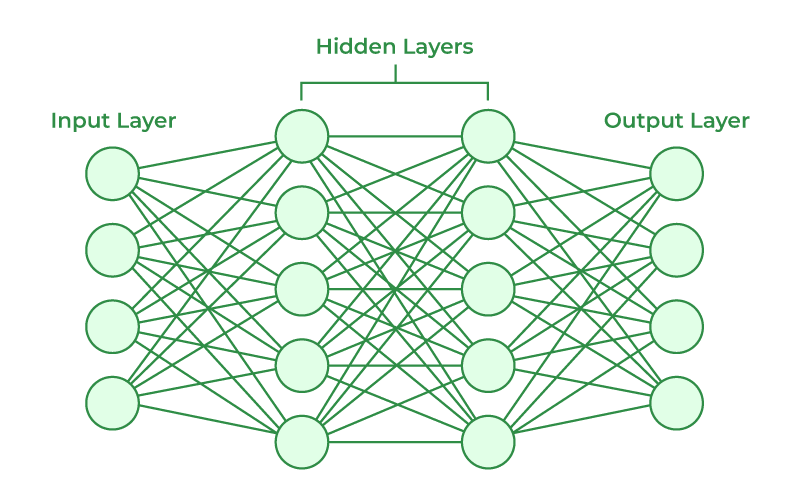
\includegraphics[width=0.55\linewidth]{annpod_fig/Neural_Network.png}
    \caption{An example neural network with input shape 3, $H=2$ hidden layers and $n=5$ neurons}
    \label{fig:neural_network}
\end{figure}


\subsection{Data Generation}
The data samples are generated through a technique called Latin Hypercube Sampling (LHS) \cite{saves2024smt}, which is a statistical method for generating a near-random sample of parameter values from multiple-dimensional space. The process ensures that each sample represents a unique combination of values across all dimensions. 

Consider the example of $N$ samples with $M$ dimensions \footnote{In our case, we chose $M=2$, the number of parameters in $\mathbf{\mu}$}, each parameter dimension is divided into $N$ equal intervals. Within each interval along each dimension, one point is randomly selected, and the samples within each dimension are randomly shuffled. Finally, the shuffled samples from each dimension are randomly combined to obtain the final set of $N$ Latin hypercube samples. LHS reduces systematic bias due to the sequential generation of samples through shuffling, while preserving the generality by considering samples across the whole interval within each dimension. 

The LHS has provided us with a random set of input parameters. We could then calculate the corresponding outputs of shape $L$ by solving for the high-fidelity FEM solutions and project them onto the reduced basis space $\mathbf{V}_{rb}$ using the method described in Section 4. 

\subsection{Feature Scaling}
Feature scaling is a method in data preprocessing that aims to normalise the values of variables within a dataset. This approach makes the data comparable on a similar scale and prevents any single feature from overshadowing others due to its larger values. In this project, the simple Min-Max Scaling scheme is used, where the data are scaled linearly based on a predefined range, usually determined by the activation function used \footnote{In this project, we mostly used the scaling range [0,1] with the sigmoid activation function or [-1, 1] with the tanh-hyperbolic activation function}. For a data set where the minimum and maximum values are $\mu_{min}$ and $\mu_{max}$, and the scaled range is $[a, b]$, each input $\mu_i$ can be scaled as:

\begin{equation}
    \mu^{norm}_i = \left( b - a \right) \times \frac{\mu_i - \mu_{min}}{\mu_{max} - \mu_{min}} + a
    \label{eqn:data_scaling}
\end{equation}

Note that the input $\bm{\mu}$ in our case has two dimensions, so each dimension is scaled independently using Equation \ref{eqn:data_scaling}. In addition, Equation \ref{eqn:data_scaling} also defines the way of reconstructing the original $\mu_i$ using the scaled value $\mu^{norm}_i $, as well as the scaling range defined by $[\mu_{min}, \mu_{max}]$.

\subsection{Training of ANN}
In this project, we used a feed-forward ANN with $H$ hidden layers, each of $n$ neurons.  The $N$ samples of data points are randomly split into an 80\% group for training and a 20\% group for validation purposes. The training dataset is also grouped into batches to speed up the training of the ANN, which means that the losses are summed up within each batch before performing backward propagation for gradient optimisation.  

In training the ANN, we used the Adam optimiser with different learning rates, with the optimal choice tuned through trials and errors.  For the loss function, we firstly tried the mean absolute error(MAE), which measures the mean of the sum of the absolute difference of the coefficients between the predicted results and the original reduced basis coefficients for each mode:

\begin{equation}
    \text{MAE} = \frac{1}{N} \sum_{n=1}^{N} \sum_{l=1}^{L} | s_l^{(n)} - \hat{s_l}^{(n)}|
\end{equation}

Another common choice for the error function was the mean squared error (MSE), which is defined as follows:

\begin{equation}
    \text{MSE} = \frac{1}{N} \sum_{n=1}^{N} \sum_{l=1}^{L} \left( s_l^{(n)} - \hat{s_l}^{(n)} \right)^2
\end{equation}

Both choices of loss functions were implemented and compared, and eventually, the MSE was preferred. In our case, we decided to place more tolerance on smaller localised errors. Since MSE squares the errors before averaging them, it penalises large errors more heavily than smaller ones. This property makes MSE particularly useful in scenarios where it is important to minimise the impact of outliers or large errors, as it prioritizes reducing these errors to improve overall performance. Additionally, the mathematical properties of MSE, such as differentiability, make it well-suited for optimisation. A more quantitative comparison will also be provided in Section 6.

To terminate the training of the ANN, we introduced two stopping criteria. The first one is simply the maximum number of training epochs, and the training stops if the number of training iterations exceeds the limit. The second one is the early-stopping criterion with a tolerance of 3 training epochs. This means that if there are no improvements in the validation data loss for 3 consecutive iterations, we would stop the training process and the model parameters at the point of early stopping are retained as the final model. The early-stopping criterion is a regularisation technique that prevents overfitting of the training data and improves its generalisation ability to unseen data., while the incorporated tolerance also gives a chance for the optimisation process to escape from the local optimum.  

Batch normalisation was also used in the training process. It normalises the inputs of each layer in a neural network to have a mean of zero and a standard deviation of one. This is done by adjusting the activations using the mean and variance calculated over the current mini-batch. For each batch during training, before passing the inputs to the next layer, batch normalization computes the mean ($\mu_B$) and variance ($\sigma^2_B$) of the activations along each feature dimension. The activations for each feature are normalised using the mean and variance obtained from the mini-batch using $\hat{x}_i = \frac{x_i - \mu_B}{\sigma_B}$.

The batch normalisation helps stabilise and speed up the training of deep neural networks by reducing internal covariate shifts. In addition, it allows for the use of higher learning rates, which can accelerate convergence during training.

With the help of the ANN, the original PDE can now be solved in a data-driven approach, and knowledge of the original problem (i.e. the governing equations, weak forms etc) is no longer needed. This greatly simplifies the computation, with some sacrifice on the solution accuracy. 

The effectiveness of ANN depends heavily on the choices of hyperparameters including the learning rate, the number of neurons per layer $n$ and the number of hidden layers $H$. To evaluate the performance of the ANN, an approach similar to the one used for evaluating POD was used. New testing samples of inputs were randomly initialised and solved with ANN for the predicted solution on the reduced space, as well as the FEM method for the high-fidelity solution. The ANN solutions were then reconstructed using $\mathbf{u}_{rb}$, and the relative error could be calculated against the high-fidelity FEM solution. This allows us to examine the performance of the trained ANN model. Optimal choices of these hyperparameters were discovered through trials and errors. Details of the results can be found in the next section. 

\subsection{Parameter Range}
Another important aspect of concern is the range of each parameter. In all cases, the input parameters \footnote{These include the input parameters generated for POD to form the reduced basis, training and validation data for the ANN, as well as the testing data for the final model.} are generated within the input range we define. These ranges also determine the scaling in equation \ref{eqn:data_scaling}. Initially, we kept an arbitrarily general range for both $\mu_1$ and $\mu_2$. This was during the later part of the project refined to $\mu_1 \in [2\pi, 2.5\pi]$ and $\mu_2 \in [12, 13]$, where an acceptable level of accuracy could be achieved from the trained model with a reasonably low number of training samples needed. Ideally, we would like as wide a range as possible (and within a physical sense) to improve the generality of the ANN-POD model. However, the actual performance might be limited, and a wider range of parameters would require a more complex model, more training data and training time, which was not further discovered due to the limited computational resources and time of this project. 

\newpage